\documentclass[pdftex,12pt,a4paper,twoside,openright]{report}

% Aaron Snsowell Thesis Document

\usepackage[rmargin=2cm,lmargin=3cm,tmargin=2cm,bmargin=2cm]{geometry}
\usepackage{setspace}
\usepackage{framed}
\usepackage[usenames,dvipsnames]{xcolor}
\usepackage{framed}
\usepackage{fancybox}
% Used for images
\usepackage[pdftex]{graphicx}
% Used to get nice (r) and (c) symbols
\usepackage{textcomp}
% Used for equations
\usepackage{mathtools}
% Used for headers
\usepackage{fancyhdr}
% Used for referencing sections
\usepackage{nameref}
% Used for nice " and ' quotes
\usepackage{csquotes}
% Used to refer to things using their names
\usepackage{nameref}
% Used for highlighting TODO sections
\usepackage{soul}
% Used for nice captions
\usepackage{caption} 
% Used to force figures to be in their respective sections
\usepackage[section]{placeins}

% Set up caption spacing
\captionsetup[table]{skip=2pt}
\captionsetup[figure]{skip=2pt}

% Set image path
\graphicspath{{./images/}}

% Penalise orphans (singe lines at the bototm of a page)
% and widows (single lines at the bottom of a page)
\widowpenalty=10000
\clubpenalty=10000

% Set spacing and 'graph indentation
\doublespacing
\setlength{\parindent}{1.5cm}


% Horizontal rule command
\newcommand{\HRule}{\rule{\linewidth}{0.5mm}}

% Nice tilde command
\newcommand{\nicetilde}{{\raise.17ex\hbox{$\scriptstyle\mathtt{\sim}$}}}

% Set up headers
\pagestyle{fancy}
\renewcommand{\headrulewidth}{0.1pt}
\renewcommand{\chaptermark}[1]{\markboth{#1}{}}
\renewcommand{\sectionmark}[1]{\markright{#1}{}}

\fancyhead[RE, LO]{}
\fancyhead[RO]{\small \leftmark~(\rightmark)}
\fancyhead[LE]{\small Light Field De-blurring for Robotics Applications}
\fancyfoot[c]{\small \thepage}

\begin{document}

% Title page

\begin{titlepage}

\begin{center}

% Upper part of the page
\includegraphics[width=4cm]{UQ.png}\\[1.5cm]    

\textsc{\Large \bfseries {\Huge T}HE {\Huge U}NIVERSITY OF {\Huge Q}UEENSLAND}\\[2cm]

\textsc{\large \bfseries Bachelor of Engineering Thesis}\\[1.5cm]


\newlength{\mylength}

\setlength{\fboxsep}{1pt}
\setlength{\mylength}{\linewidth}

\addtolength{\mylength}{-1.5\fboxsep}
\addtolength{\mylength}{-1.5\fboxrule}

\doublebox{%
\parbox{\mylength}
{
\begin{center}
\large Light Field Deblurring for Robotics Applications
\end{center}
}
}

		
\textsc{}\\[1.5cm]

% Author and supervisor
\begin{minipage}{0.8\textwidth}
\begin{flushleft} \large
Student Name: \textsc{Aaron Snoswell}\\[0.1cm]
Course Code: METR4901\\[0.1cm]
Supervisor: Dr. Surya P. N. Singh\\[0.1cm]
Submission Date: 16 June 2014\\[0.1cm]
\end{flushleft}
\end{minipage}




\vfill


{\small A thesis submitted in partial fulfilment of the requirements of the\\
Bachelor of Engineering Degree in Mechanical Engineering\\[1.5cm]}

\textcolor{Gray}
{
{\small  \bfseries UQ Engineering\\[0.5cm]
Faculty of Engineering, Architecture and Information Technology}
}


\end{center}

\end{titlepage}

\clearpage{\thispagestyle{empty}\cleardoublepage}
\thispagestyle{empty}

\begin{flushright}

Aaron Snoswell

Student Number: 42028563

2 Hamilton Rd \\
Wavell Heights \\
QLD Australia, 4012
\end{flushright}


\begin{flushleft}

Monday, 16\textsuperscript{th} June, 2014

\bigskip

Prof. Paul Strooper \\
Head of School \\
School of Information Technology and Electrical Engineering \\
The University of  Queensland \\
St Lucia QLD 4072 \\

\vspace*{\baselineskip}
Dear Professor Strooper,

\vspace*{\baselineskip}
In accordance with the requirement of the Degree of Bachelor of Engineering (Honours) in the School of Information Technology and Electrical Engineering, I submit the following thesis entitled
\begin{center}

\enquote{Light Field De-blurring for Robotics Applications}

\end{center}
The thesis was performed under the supervision of Dr. Surya P. N. Singh. I declare that the work submitted in this thesis is my own, except as acknowledged in the text and footnotes, and has not been previously submitted for a degree at the University of Queensland, or any other institution.

\vspace*{\baselineskip}

Yours sincerely,


\medskip
\includegraphics[width=5cm]{sig.png}

Aaron Snoswell

\end{flushleft}


% Other pages

\newgeometry{
	top=2cm,
	bottom=2cm,
	lmargin=2cm,
	rmargin=3cm
}
\begin{abstract}


\begin{description}

\item[Aim:]
The aim of this research was to explore ways to restore motion-blurred Light Field (LF) images, specifically in a robotic environment.

\item[Technical Gap:]
LF cameras have a range of uses in robotics, however the performance of robotic systems can be affected by motion blur in an image.
Normal deconvolution de-blurring is limited in that it only works for images with one depth.

\item[Method:]
A well-known mathematical de-blurring technique, known as deconvolution, was adapted to work with LF images.
In this context LF images are characterised as containing x, y, colour and angular light information.

\item[Results:]
A depth-aware deconvolution technique that operates on LF images was developed.

\item[Conclusion:]
In this thesis we show how deconvolution can be applied to LF images, even when there is a range of depths within the image. The angular information available in the LF allows for depth-aware deconvolution, recovering sharp edges at all scene depths.

\end{description}

\end{abstract}

\newgeometry{
	top=2cm,
	bottom=2cm,
	lmargin=3cm,
	rmargin=2cm
}
\renewcommand{\abstractname}{Acknowledgements}
\begin{abstract}

I would like to thank my supervisor, Dr. Surya Singh for his support, patience, encouragement and advice.
His vast engineering knowledge provided many an answer, and his sense of humor many a needed laugh.

I would like to thank my wife, Centaine for the sleepless hours spent staying up with me, encouraging me to \enquote*{just write one more section}.
For all the craziness you put up with I am truly indebted to you.
To my family also; Mum, Dad, Michelle, my brothers and Candy for the love and support.
Thanks especially to Elijah, for many interesting conversations and insights from a photographer's point of view.

Thanks is owed to Donald Dansereau from the University of Sydney for his excellent work on the Light Field Toolbox for Matlab.

Thanks to the other Mechatronics staff at UQ, especially Dr. Paul Pounds and Dr. Hanna Kurniawati for your input, and Prof. Ross McAree for the support.

Finally, to the Big G upstairs, thanks for getting me this far, I couldn't have done any of it without you.

\end{abstract}

\clearpage{\thispagestyle{empty}\cleardoublepage}
\setcounter{page}{1}
\tableofcontents

\begingroup
\let\clearpage\relax
\thispagestyle{plain}
\listoffigures
\thispagestyle{plain}
\listoftables
\endgroup


\clearpage{\thispagestyle{plain}\cleardoublepage}

\chapter{Introduction}
\label{chap:introduction}

\section{Problem Statement}
\label{sec:problem_statement}

Light field cameras are a revolutionary new type of imaging device that allow four-dimensional light data to be captured.
Unfortunately, like traditional photos, light field images suffer from motion blur under certain conditions.
In this thesis we present a novel adaptation of existing de-blurring methods that allows light field images to be de-blurred, even for scenes with significantly varying depths.

\section{Technical Gap}
\label{sec:technical_gap}

Existing deconvolution de-blurring methods have the significant drawback that they only work for scenes with a constant depth.
Additionally, the application of deconvolution methods to light field images is yet to be documented in computer vision literature\footnote{Light field deconvolution has received limited attention regarding light field microscopy \cite{levoy2006microscopy}, however no documented evidence could be found regarding the use of deconvolution for \emph{de-blurring} a motion-blurred light field.}.

Light field images are of interest due to the many innovative applications they enable.
For example, light field cameras are presently popular for the ability to refocus images in software (e.g. the Lytro camera), however their applications for robotics are yet to be fully realised.
Potential robotic applications include the ability to reduce the effects of fog, snow and other partial occluders \cite{dansereau2013plenoptic}, excellent low light performance and the ability to recover depth information from a compact sensor.

Unfortunately, there are many robotic vision algorithms that rely on high-frequency image details to operate (for example any method relying on dense pixel matching or edge, line or shape detection).
Motion blur obscures this high frequency content, and has the potential to limit the performance of these methods.
In addition to this, there are many robotic scenarios where deconvolution de-blurring is inappropriate, due to the presence of large scene depth variation (e.g. ground or underwater vehicles).
With these two limitations in mind, the aim of our research was to;

\begin{enumerate}
\item Explore means for de-blurring a motion-blurred light field image, and
\item Do this, even in the presence of significant scene depth variation.
\end{enumerate}

\section{The Menu}
\label{sec:the_menu}

We begin in Chapter \ref{chap:plenoptic_deblurring} by giving an overview of the relevant theory of light field imaging.
A theoretical means for de-blurring a light field is described in Section \ref{sec:motion_blur_formation}.
This method is derived from a discussion of the formation of motion blur within a simplified camera and criticality, relies on the availability of a calibrated depth map.
Section \ref{sec:light_field_depth_estimation} provides this key by discussing the problem of estimating depth from a light field image and calibrating this depth information to metric units.
The ability to obtain calibrated depth maps from a light field concludes the theoretical section of this document and provides a complete framework for what we call \enquote*{depth-aware deconvolution} - that is, de-blurring a light field image at all scene depths.

Chapter \ref{chap:experimental_method} describes our experiment, designed to test the simplified case of linear camera motion blur in shallow-depth, controlled environments.
Chapter \ref{chap:results_and_discussion} details the success of our method, and highlights the potential applications, as well as the limitations and assumptions made.
In addition, a number of areas for future research are identified.


\chapter{Plenoptic De-blurring}
\label{chap:plenoptic_deblurring}

\section{Light Field Theory}
\label{sec:light_field_theory}

The light field is a mathematical description of the way light propagates.
Another name for this is the \enquote*{Plenoptic Function}, from the Latin \enquote*{plenus}, meaning full, and \enquote*{optic}, meaning light.
The plenoptic function describes every possible configuration a light ray could ever be in, encompassing the three spatial dimensions, two angular dimensions, temporal changes as well as frequency (colour), phase and polarisation changes.
In most computer vision literature the phase and polarisation elements are ignored, leading to a 7-dimensional definition of the plenoptic function;

\begin{equation}
\label{eq:plenoptic_function}
P = P(V_x, V_y, V_z, \theta, \phi, t, \lambda)
\end{equation}

\noindent
where $V_x$, $V_y$ and $V_z$ are the spatial dimensions, $\theta$ and $\phi$ are the angular dimensions, $t$ is the temporal dimension and $\lambda$ describes the colour of the ray. 

The plenoptic function in this form was first described by Adelson and Bergen in 1991 \cite{adelson1991plenoptic}.
Adelson and Bergen developed a light field theory by asking the fundamental question \enquote{What can be seen?} They stressed that the plenoptic function is the sole visual communication link between physical objects and the eye.
They also suggested that the function of \enquote*{early vision} in biological and artificial organisms is to sample the derivative of this function along various dimensions such as \enquote*{change in colour with x} or \enquote*{change in brightness with time}.

In computer vision literature, many different representations of the light field have been proposed, each emphasising different aspects of the plenoptic function.
McMillan and Bishop discuss the representation of 5D light field images ($V_x$, $V_y$, $V_z$, $\theta$ and $\phi$) as a set of multiple panoramic images taken at different physical locations \cite{mcmillan1995plenoptic}.
Importantly, in free-space (space free of occluding objects), one of the spatial dimensions is redundant, a consequence of the fact that radiance does not change along a line unless blocked \cite{levoy1996light}.
Thus, for free space, the 5th light field dimension can be dropped, giving a 4D light field definition.

Levoy and Hanrahan describe a parameterisation for the 4D light field which they term a \enquote*{light slab} \cite{levoy1996light}.
In this parameterisation, they describe a light ray by it's intersection through two arbitrarily placed planes in world space (Figure \ref{fig:light_slab}).

\begin{figure}[h]
\centering
\includegraphics[width=12cm]{light_slab.pdf}
\caption[The Light Slab Parameterisation of a 4D Light Field]{
The Light Slab Parameterisation of a 4D Light Field, described by Levoy and Hanrahan \cite{levoy1996light}.
A light ray is defined as passing through two arbitrary planes in world-space.
By their convention, both planes range from 0 to 1, and the dimensions are labeled $u$ and $v$, and $s$ and $t$ for the first and second planes respectively.
}
\label{fig:light_slab}
\end{figure}

The light slab parameterisation is useful as is similar to the design used in many modern light field cameras.
Traditional cameras generally sample the Light Field along two dimensions (x and y pixel locations) and in the colour dimension.
This is done using a 2D array of light-sensitive pixel elements, masked in a pattern to detect different light wavelengths (normally corresponding with the colours \enquote*{Red}, \enquote*{Green} and \enquote*{Blue}).
While there is active research in developing angle-sensitive pixels \cite{wang2009angle, wang2011angle, wang2012angle}, most modern light field cameras encode angular information by mapping ray angles to 2D sensor array locations, sacrificing spatial resolution for angular resolution.

Such cameras were first envisaged in 1996; independent research by Gortler et al. and Levoy et al. suggested it was possible to capture 4D light field information using a traditional camera sensor with some modifications \cite{gortler1996lumigraph, levoy1996light}.
Such a camera was physically constructed recently by Ren Ng and is described in his dissertation \cite{ng2006digital}.
Ng's prototype light field camera used a microlens array placed over a regular DSLR camera sensor \cite{ng2006digital}.
This design mirrors the light slab parameterisation, with one plane being placed in front of the camera, and one plane inside the camera body \cite{dansereau2013plenoptic}.
Based on his research, Ng went on to found Lytro inc. and developed the consumer oriented Lytro light field camera, which is used in our experiments.

As stated above, the Lytro is based on the principle of sacrificing spatial resolution for angular resolution.
The Lytro has an 11 mega-pixel sensor chip, however a spatial and angular resolution of only 1080x1080 and 10x10 respectively \cite{lytro2014techspecs}.
The trade-off between angular resolution and spatial resolution is unavoidable when using this type of camera design, and the choice of which light field dimensions to sample limits the practical functions that can be performed with the captured light field.

Other ways of sampling the 4D light field include using an array of curved mirrors to reflect light \cite{nayar2004programmable}, using a pinhole mask to refract light \cite{veeraraghavan2007dappled}, using multiple traditional cameras separated spatially in a grid \cite{wilburn2005high}, or multiple photographs separated temporally \cite{levoy1996light}.
Additionally, Google recently announced an update for Android based smartphones that enables limited light field photography in a mobile device for the first time, by taking multiple photos separated spatially \cite{google2014lensblur}.

In methods that trade spatial resolution for angular resolution, the images that can be formed by slicing the light field are unavoidably of a much lower resolution than regular cameras.
To this end, recent research by Bishop et al. has demonstrated so-called \enquote*{Light Field Superresolution} \cite{bishop2009light}.
This and other related techniques incorporate image priors such as scene lambertianty and texture statistics to boost the apparent resolution of the re-constructed images through a Bayesian statistical framework.

For our experiments we used the Lytro camera to capture light field images.
By studying the way motion blur forms in a camera (Section \ref{sec:motion_blur_formation}), we develop a means for de-blurring images (light field or otherwise) at all scene depths.
This technique relies on the availability of a calibrated depth map, and the Lytro camera is used to supply this depth data.
By demonstrating a means for de-blurring light field images it is hoped that light field sensors will see increased usefulness as tools for robotic navigation and in computer vision applications.

\section{Motion Blur Formation}
\label{sec:motion_blur_formation}

In order to de-blur a light field, it is necessary to understand the way motion blur forms in an optical system.
Motion blur occurs in any non-theoretical camera due to a finite exposure time combined with the presence of camera, or object motion.
This is distinct from focal blur, which is a by-product of the optical behavior of any camera aperture larger than an infinitesimal point (a perfect pinhole aperture).
If the camera or objects within the scene move during the exposure time, light rays from the scene that would otherwise be focused on a single photosite are distributed across multiple photosites.
The objects within the scene therefore become \enquote*{smeared} across several pixels in the resultant image (Figure \ref{fig:integration_blur}).

\begin{figure}[h]
\centering
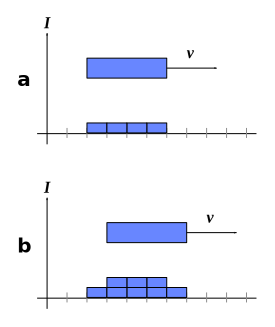
\includegraphics[width=8cm]{integration_blur.pdf}
\caption[Motion Blur Caused by Camera Integration]{
a) In this simplified, orthographic-projection camera, photosites integrate the scene intensity vertically ($I$) b) When the object moves at during the image exposure, the light from the object is distributed across multiple photosites, resulting in motion blur.
}
\label{fig:integration_blur}
\end{figure}

In a projective geometry imaging system, such as most cameras, blur from camera or object linear motion in any plane perpendicular to the optical axis appears as a linear \enquote*{smear} in the image x or y directions.
This \enquote*{smear} is known as a Point Spread Function (PSF), as it describes the spreading that occurs to the image of a perfect point source within the scene.
This is analogous to the impulse response of a frequency domain system; in this case the system is the optical apparatus, and the impulse is the point source in the scene.

Movement along the optical axis results in a radially varying PSF, while camera or object rotation creates a more complex PSF again.
In all cases, the degree of blur varies with the distance from the camera to the object moving.
For the sake of simplicity, in the experiments performed here we focus only on de-blurring linear motion blur induced through camera motion.

In order to de-blur light field data, it was necessary to quantitatively describe the way motion blur forms in a camera.
Specifically, it was necessary to derive an equation describing the way a motion blur PSF varied with respect to scene depth.
To do this, the homogeneous projective geometry equation was used;

\begin{equation}
\label{eq:camera_projection_unexpanded}
k \boldsymbol{x} = \boldsymbol{K} \left[~\boldsymbol{R}~|~\boldsymbol{t}~\right] \boldsymbol{X}
\end{equation}

\noindent
where $k$ is the homogeneous scaling constant, $\boldsymbol{x}$ is the image-space point location, $\boldsymbol{K}$ is the so-called \enquote*{camera intrinsic matrix} that accounts for camera distortions, $\boldsymbol{R}$ is the 3x3 camera rotation matrix,  $\boldsymbol{t}$ is the camera's 3x1 world-frame translation vector and $\boldsymbol{X}$ is the world-frame point location.

Expanding the matrix and vector terms, equation \ref{eq:camera_projection} is reached.

\begin{equation}
\label{eq:camera_projection}
k
\begin{bmatrix}
x \\
y \\
1 \\
\end{bmatrix}
=
\begin{bmatrix}
\alpha && s && u_0 \\
0 && \beta && v_0 \\
0 && 0 && 1 \\
\end{bmatrix}
\begin{bmatrix}
r_{11} && r_{12} && r_{13} && t_x \\
r_{21} && r_{22} && r_{23} && t_y \\
r_{31} && r_{32} && r_{33} && t_z \\
\end{bmatrix}
\begin{bmatrix}
X \\
Y \\
Z \\
1
\end{bmatrix}
\end{equation}

Here the intrinsic matrix $\alpha$ and $\beta$ terms are the camera focal length, scaled to be in units of x and y pixels respectively, $s$ is a shearing factor that describes the shear of the camera sensor (see Figure \ref{fig:intrinsic_shear}) and $u_0$ and $v_0$ are the x and y pixel locations of the optical axis of the camera.

\begin{figure}[h]
\centering

\includegraphics[width=4cm]{pixel_shear.pdf}
\caption[Camera intrinsic matrix shear term]{Camera intrinsic matrix shear term description, $s = \beta\tan(\theta)$. Figure from \cite{pollefeys2002visual}}
\label{fig:intrinsic_shear}
\end{figure}

Assuming the world frame coincides with the camera location and orientation, and assuming linear, horizontal camera motion at velocity $v_c$ meters per second with an exposure time of $t_e$ seconds, the blur width of a point source in the scene can be derived;

\begin{align}
w &= \left| x_1 - x_2 \right| \notag \\
&= \left| \left( \frac{\alpha + s + u_0}{Z} \right) X_1 - \left( \frac{\alpha + s + u_0}{Z} \right) X_2 \right| \notag \\
&= \left| \left( \frac{\alpha + s + u_0}{Z} \right) \left(\frac{- v_c t_e}{2}\right) - \left( \frac{\alpha + s + u_0}{Z} \right) \left(\frac{v_c t_e}{2}\right) \right| \notag \\
\label{eq:blur_width_full}
&= \left( \frac{\alpha + s + u_0}{Z} \right) v_c t_e
\end{align}

Finally, if we then assume square sensor pixels with no sensor skew, and an aligned optical axis, equation \ref{eq:blur_width_full} simplifies to

\begin{equation}
\label{eq:blur_width_simple}
w = \frac{f}{Z} v_c t_e
\end{equation}

\noindent
where $f$ is the focal length of the camera.
This equation describes the width of the linear motion blur created by a point source at depth $Z$ within the scene for a moving camera.
Note that the blur width is proportional with the camera focal length, velocity and exposure time, and inversely proportional with depth.
The inverse relation with scene depth correlates with the intuitive expectation; objects further away translate less in an image when the camera moves.
Equation \ref{eq:blur_width_simple} can be thought of as describing a 3D point spread function with $x$, $y$ and $Z$ as the dimensions.
This is shown visually in Figure \ref{fig:psf_3d}.


\begin{figure}[h]
\centering
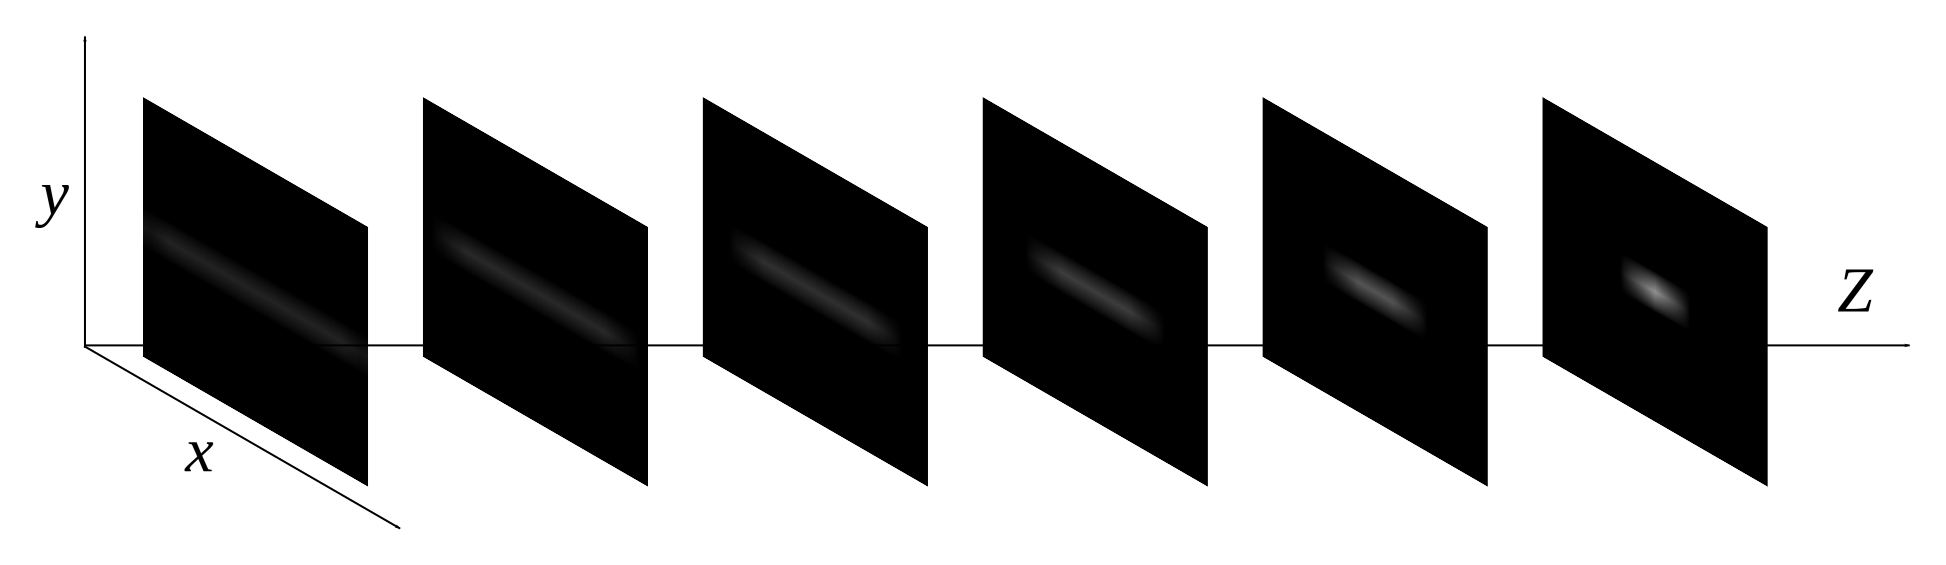
\includegraphics[width=\textwidth]{psf_3d.pdf}
\caption[Visualisation of a 3D Point Spread Function]{Visualisation of a 3D Linear Motion Point Spread Function, with $x$, $y$ and $Z$ as the dimensions}
\label{fig:psf_3d}
\end{figure}

Equation \ref{eq:blur_width_simple} was verified experimentally by taking several photos with a Lytro camera at a controlled velocity and measuring the blur width and depth of objects within the scene.
Only the central sub-aperture image from the light field was used for simplicity.
Figure \ref{fig:blur_vs_depth} shows the measured results along with the predicted curve.

\begin{figure}[h]
\centering
\includegraphics[width=\textwidth]{blur_vs_depth.pdf}
\caption[Edge Blur Width vs. Depth]{
Edge Blur Width vs. Depth - Measured and Predicted
}
\label{fig:blur_vs_depth}
\end{figure}

As can be seen, the equation matched the theoretical curve very closely, indicating that Equation \ref{eq:blur_width_simple} is a good fit for an individual sub-aperture image within a Lytro light field.
This shows that if the focal length, linear camera velocity and exposure time are known, and if a calibrated depth map can be recovered from the light field, it should be possible to de-blur all sub-aperture images from the light field image at all scene depths.
This is the basis for the light field de-blurring technique developed here.
As a final note, observe that the above analysis could also be applied to compute the 3D point spread function for a general camera trajectory, provided the trajectory (camera $\boldsymbol{R}$ and $\boldsymbol{t}$ at all times during the exposure) was known.
This possibility is discussed further in Chapter \ref{chap:results_and_discussion} (\nameref{chap:results_and_discussion}).


\section{Image De-blurring}
\label{sec:image_deblurring}

Knowledge of the way blur forms in a camera is pointless without a means to remove this blur.
There are several techniques used to remove the effects of motion and focal blur, the most common of which involve deconvolution.

As discussed in Section \ref{sec:motion_blur_formation}, motion blur is formed by camera or object movement during the camera exposure.
This is equivalent to convolution of a true image $f$ with the blur kernel or \enquote*{Point Spread Function} $g$.

\begin{equation}
\label{eq:spatial_blur_simple}
i(x) = f(x)~\textasteriskcentered~g(x)
\end{equation}

Writing this in the frequency domain, we get

\begin{equation}
\label{eq:frequency_blur_simple}
I(f) = F(f) \times G(f)
\end{equation}

\noindent
where $I$ is the observed image, $F$ is the original image and $G$ is the Fourier transform of the PSF, the so-called Optical Transfer Function (OTF).
Note that in the frequency domain, the convolution operator (\textasteriskcentered) is a simple element-wise multiplication and is therefore computationally fast.
This is the reason most image de-blurring techniques are performed in the frequency domain.

Supposing that the function $G$ can be found, it should theoretically be possible to recover the true image using

\begin{equation}
\label{eq:frequency_blur_inverse_simple}
F(f) = \frac{I(f)}{G(f)}
\end{equation}

\noindent
where element-wise division is used, and the inverse Fourier transform of $F$ is taken.
Unfortunately, in practice this is not possible for two reasons; firstly, $G$ will contain zeros that cause the values of $F$ to go to infinity.
Secondly, in practice the imaging system is subject to noise, indicated by $n$ (or $N$ in the frequency domain).
This can come in the form of Poisson shot noise, caused by the quantum nature of light, as well as device-specific detection noise.

\begin{equation}
\label{eq:frequency_blur_full}
I(f) = F(f) \times G(f) + N(f)
\end{equation}

These two factors mean that recovering the true image $f$ is not possible in practice.
Deconvolution de-blurring methods are an attempt to find a function $f'$ that estimates $f$ as accurately as possible, whilst being robust to the presence of additive noise.

De-convolution methods can be divided into several categories.
Linear deconvolution methods are most similar in operation to Equation \ref{eq:frequency_blur_inverse_simple}.
The most naive deconvolution is a regularised form of Equation \ref{eq:frequency_blur_inverse_simple}, where values in $F$ that would otherwise be infinite (due to zeros in $G$) are set to 0;

\begin{equation}
\label{eq:regularised_deconvolution}
F(f) = \begin{cases}
	\frac{I(f)}{G(f)},	& \left| H(f) \right| \ge \epsilon> 0 \\
	0					& \text{otherwise}
\end{cases}
\end{equation}

This is sometimes known as \enquote*{stabilised} deconvolution.
Note that regularised deconvolution does nothing to account for noise in the image, and will therefore \enquote*{amplify} the presence of noise in the recovered image $f'$.

Wiener filtering improves on this and is a general signal processing technique that attempts to recover an estimate of a signal in the presence of additive noise \cite{wiener1964extrapolation}.
Applied to image processing, Wiener deconvolution can be written as

\begin{equation}
\label{eq:wiener_filter}
F(f) = I(f) \left( \frac{G(f)^* \hat{I}(f)}{\left| G(f) \right|^2 \hat{I}(f) + \hat{N}(f) } \right)
\end{equation}

\noindent
where $\hat{I}$ and $\hat{N}$ are the mean spectral power densities of observed image $i$ and the noise $n$ respectively and $*$ denotes complex conjugation.
As can be seen, at frequencies with high noise, the Wiener filter suppresses the output, $F$ reducing the amplification of noise that regularised deconvolution suffers from.
Winer deconvolution has the drawback that the spectral content of the image and noise must be known, or estimated.

More complex convolution methods are framed in an iterative fashion.
These methods iteratively solve the minimisation of some cost function.
This cost function can be defined in a least-squares framework \cite{ng99anew} or as an expectation-maximisation problem, as is the case with the well known Richardson-Lucy deconvolution method \cite{richarson1972bayesian}.
This method seeks to maximise the probability of observing the image $I$ if the true image is some other trial image.

Finally, blind deconvolution methods are a collection of more recent techniques where no information about the PSF needs to be supplied \cite{bell1995information, ayers1988iterative}.
In these methods, an estimate of the original image is made, then convoled with a theoretical PSF.
This is compared with the observed image and corrections made to both the PSF and original image estimates.
The process then repeats iteratively until some stopping criterion is met.
These methods have the obvious advantage that they operate without the prior PSF.

In our experiments we apply Richardson-Lucy deconvolution to a light field image, using the depth map to vary the PSF for different parts of the scene.
Richardson-Lucy deconvolution was selected due to it's computational simplicity and robust performance in the presence of noise, however any deconvolution method could be used in it's place.
We compare the results of our depth-aware deconvolution technique with those of Regularised, Blind and 2D Richardson-Lucy deconvolution to demonstrate the improvement that using a depth-aware PSF brings.

\section{Light Field Depth Estimation}
\label{sec:light_field_depth_estimation}

As shown in section \ref{sec:motion_blur_formation}, de-blurring at all scene depths requires a depth map calibrated to be in metric units such as meters.
It was found that the Lytro firmware and/or desktop software computes a low-quality depth map from the Lytro Light Field images, returning integer depth values in an arbitrary unit.
These depth maps are located within the Lytro image storage database and are contained in Lytro image files with the name \enquote*{dm.lfp}.
The \enquote*{lfpsplitter} tool \cite{patel2013lfptools} was used to extract this data into a single-column text file format, after which Matlab was used to reshape this data into a depth map.
To correctly re-shape the data, it had to be read in standard raster order (left to right, top to bottom), with an expected size of 330x330.
In the resulting depth maps, lower (darker) values indicate objects closer to the camera.

Further research and analysis is needed to more fully quantify the Lytro depth response function, however an initial investigation was performed using several Lytro images.
Sample points from within the Lytro depth maps were compared with metric depth estimates for a range of scenes, with the scene depth ranging up to \nicetilde2.5 meters.
Our initial analysis showed that after the rejection of outliers, the Lytro depth response \enquote*{$D$} was a linear function with metric object depth \enquote*{$Z$}, however the specific linear function varied as the overall scene depth range changed.
For example, scenes with an overall depth range less than 0.5m were found to be a good fit ($R^2 = 0.69$) with the linear function $Z(D) = 0.0291 D + 0.2114$, while scenes with a depth range of 0.5-2.5m were a good fit ($R^2 = 0.7$) with the function $Z(D) = 0.1503 D + 0.781$.
More data is needed to derive a continuous function $D \Rightarrow Z$, however for simplicity the piecewise mapping described here was used in our experiments.
Figure \ref{fig:depth_real_world_vs_lytro_response} shows these results in graph format.

Thus, if prior information is available about the overall depth range of the scene ($\hat{Z}$), the Lytro depth map data can be calibrated to metric units;

\begin{equation}
\label{eq:lytro_dm_to_metric}
Z(D, \hat{Z}) = \begin{cases}
	0.0291 D + 0.2114, & \hat{Z} < 0.5m. \\
	0.1503 D + 0.781, & 0.5 \leq \hat{Z} < 2.5m. \\
\end{cases}
\end{equation}

\noindent
where $\hat{Z}$ is the \emph{a-priori} rough scene depth estimate.
Insufficient data was collected for scenes with depth beyond 2.5 meters to characterise the depth response in those regions.

It was found experimentally that the Lytro-generated depth maps have a minimum recoverable depth range of \nicetilde5cm and that the presence of glare prevents accurate depth estimation (see Figure \ref{fig:ruler_glare_min_dist}).
Furthermore, it was found that the presence of motion blur or lack of scene structure reduced the quality of the depth map (see Figures \ref{fig:depth_lack_of_structure} and \ref{fig:blur_corrupts_depth}).
The reduction in quality due to glare is expected due to the lambertian scene assumption made in many light field computational photography algorithms \cite{bishop2009light, liang2011light, baker2003shape} and the reduction in quality due to motion blur or lack of structure suggests the Lytro software is using a dense correlation based depth estimation method.

\begin{figure}[p]
\centering
\includegraphics[width=\textwidth]{depth_real_world_vs_lytro_response.pdf}
\caption[Lytro depth response vs. metric depth]{
Lytro depth response vs. metric depth.
The data has been binned into two categories based on overall scene depth range.
}
\label{fig:depth_real_world_vs_lytro_response}
\end{figure}

\begin{figure}[p]
\centering
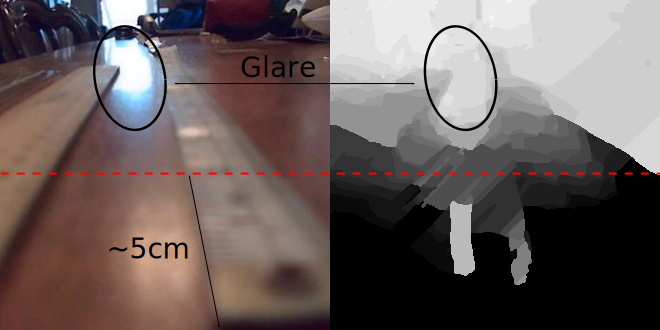
\includegraphics[width=\textwidth]{ruler_glare_min_dist.pdf}
\caption[Minimum depth map distance and the effect of glare]{
An example light field image, and the Lytro depth map response, normalised to the range [0, 1] for display.
Darker values are closer to the camera.
Note the lack of depth data where glare is present, and below Z = 5cm.
}
\label{fig:ruler_glare_min_dist}
\end{figure}

\begin{figure}
\centering
\includegraphics[width=\textwidth]{blur_corrupts_depth.png}
\caption[Motion Blur Corrupts Lytro Depth Estimation]{
The same scene photographed three times with the Lytro camera, with progressively more motion blur.
Note the reduction in the quality and consistency of the depth response.
Depth maps have been normalised to the range [0, 1] for display, and darker values are closer to the camera.
}
\label{fig:blur_corrupts_depth}
\end{figure}

These findings suggested that if rough knowledge of the scene depth could be obtained, it would possible to calibrate the Lytro depth maps into metric units.
We suggest that in a real-world application, an infra-red/ultrasound based focal length sensor (as found on many commercial cameras) could be used for this purpose.
Alternately, user-supplied a-priori knowledge of a robotic operating environment, or a user-selected \enquote*{scene} setting on a commercial camera (e.g. outdoors, indoors, portrait etc.) could be used here.

Finally, in addition to using the Lytro software depth maps, the possibility of using other depth estimation methods was explored.
In particular, the \enquote*{Depth from Combining Defocus and Correspondence} method by Tao et al. \cite{tao2013depth} was tested.
Using the supplied Matlab source code \cite{tao2013depthwebsite}, depth maps were found to be extremely noisy and completely unusable (see Figure \ref{fig:defocus_correspondence_depth}).
It is possible this was due to their code being tuned specifically for their Lytro camera, however due to discovering the more readily available Lytro depth data, this possibility was not explored further.

\begin{figure}[p]
\centering
\includegraphics[width=\textwidth]{depth_lack_of_structure.png}
\caption[Lack of Scene Structure Corrupts Lytro Depth Estimation]{
An example light field image and the Lytro depth response, normalised to the range [0, 1] for display.
Darker values are closer to the camera.
Note the lack of clear structure in some parts of the image (e.g. on the stuffed toy's face and body, and in the background) results in large regions without depth variation, despite the presence of metric depth change.
}
\label{fig:depth_lack_of_structure}
\end{figure}

\begin{figure}[p]
\centering
\includegraphics[width=7cm]{defocus_correspondence_depth.png}
\caption[Depth Map from combining Defocus and Correspondence]{
An example depth map result from using Defocus and Correspondence by Tao et al. \cite{tao2013depthwebsite}.
The input light field is the same as in Figure \ref{fig:depth_lack_of_structure}.
Darker values are supposedly closer to the camera, although the depth map does not match the real world depths.
}
\label{fig:defocus_correspondence_depth}
\end{figure}


In summary, it was found that if a rough scene depth estimate is known, the Lytro depth maps could be calibrated to metric units.
This was the final element needed to enable depth-aware deconvolution of light field images, as it allowed the blur at every point in the light field to be determined, using Equation \ref{eq:blur_width_simple}.


\chapter{Experimental Method}
\label{chap:experimental_method}

The theory derived in Chapter \ref{chap:plenoptic_deblurring} indicates that deconvolution of a light field at all scene depths should be possible. 
An experiment was designed to test this for the simplified case of linear camera motion blur with short ($<$ 0.5m) range scenes.

\section{Development of Linear Motion Platform}
\label{sec:development_of_linear_motion_platform}

A robotic linear motion platform was developed using Lego\textsuperscript{\textregistered} Mindstorms\textsuperscript{\textregistered} parts.
The platform was designed to carry a Lytro camera and a Nikon D5100 DSLR camera side-by-side.
Support for both cameras was made out of Lego parts.
The motion platform consisted of a wheeled based that carried the cameras.
It was attached by thread to a drum, driven by two Mindstorms motors.
The drum was manually held in place during operation, and the Matlab RWHT NXT Toolbox \cite{rwth2007toolbox} was used to interface with the motors.

The angular velocity of the drum was empirically calibrated allowing a desired velocity and linear distance to set in software.
Figure \ref{fig:motion_platform} shows the design of the linear motion platform.

\begin{figure}[h]
\centering
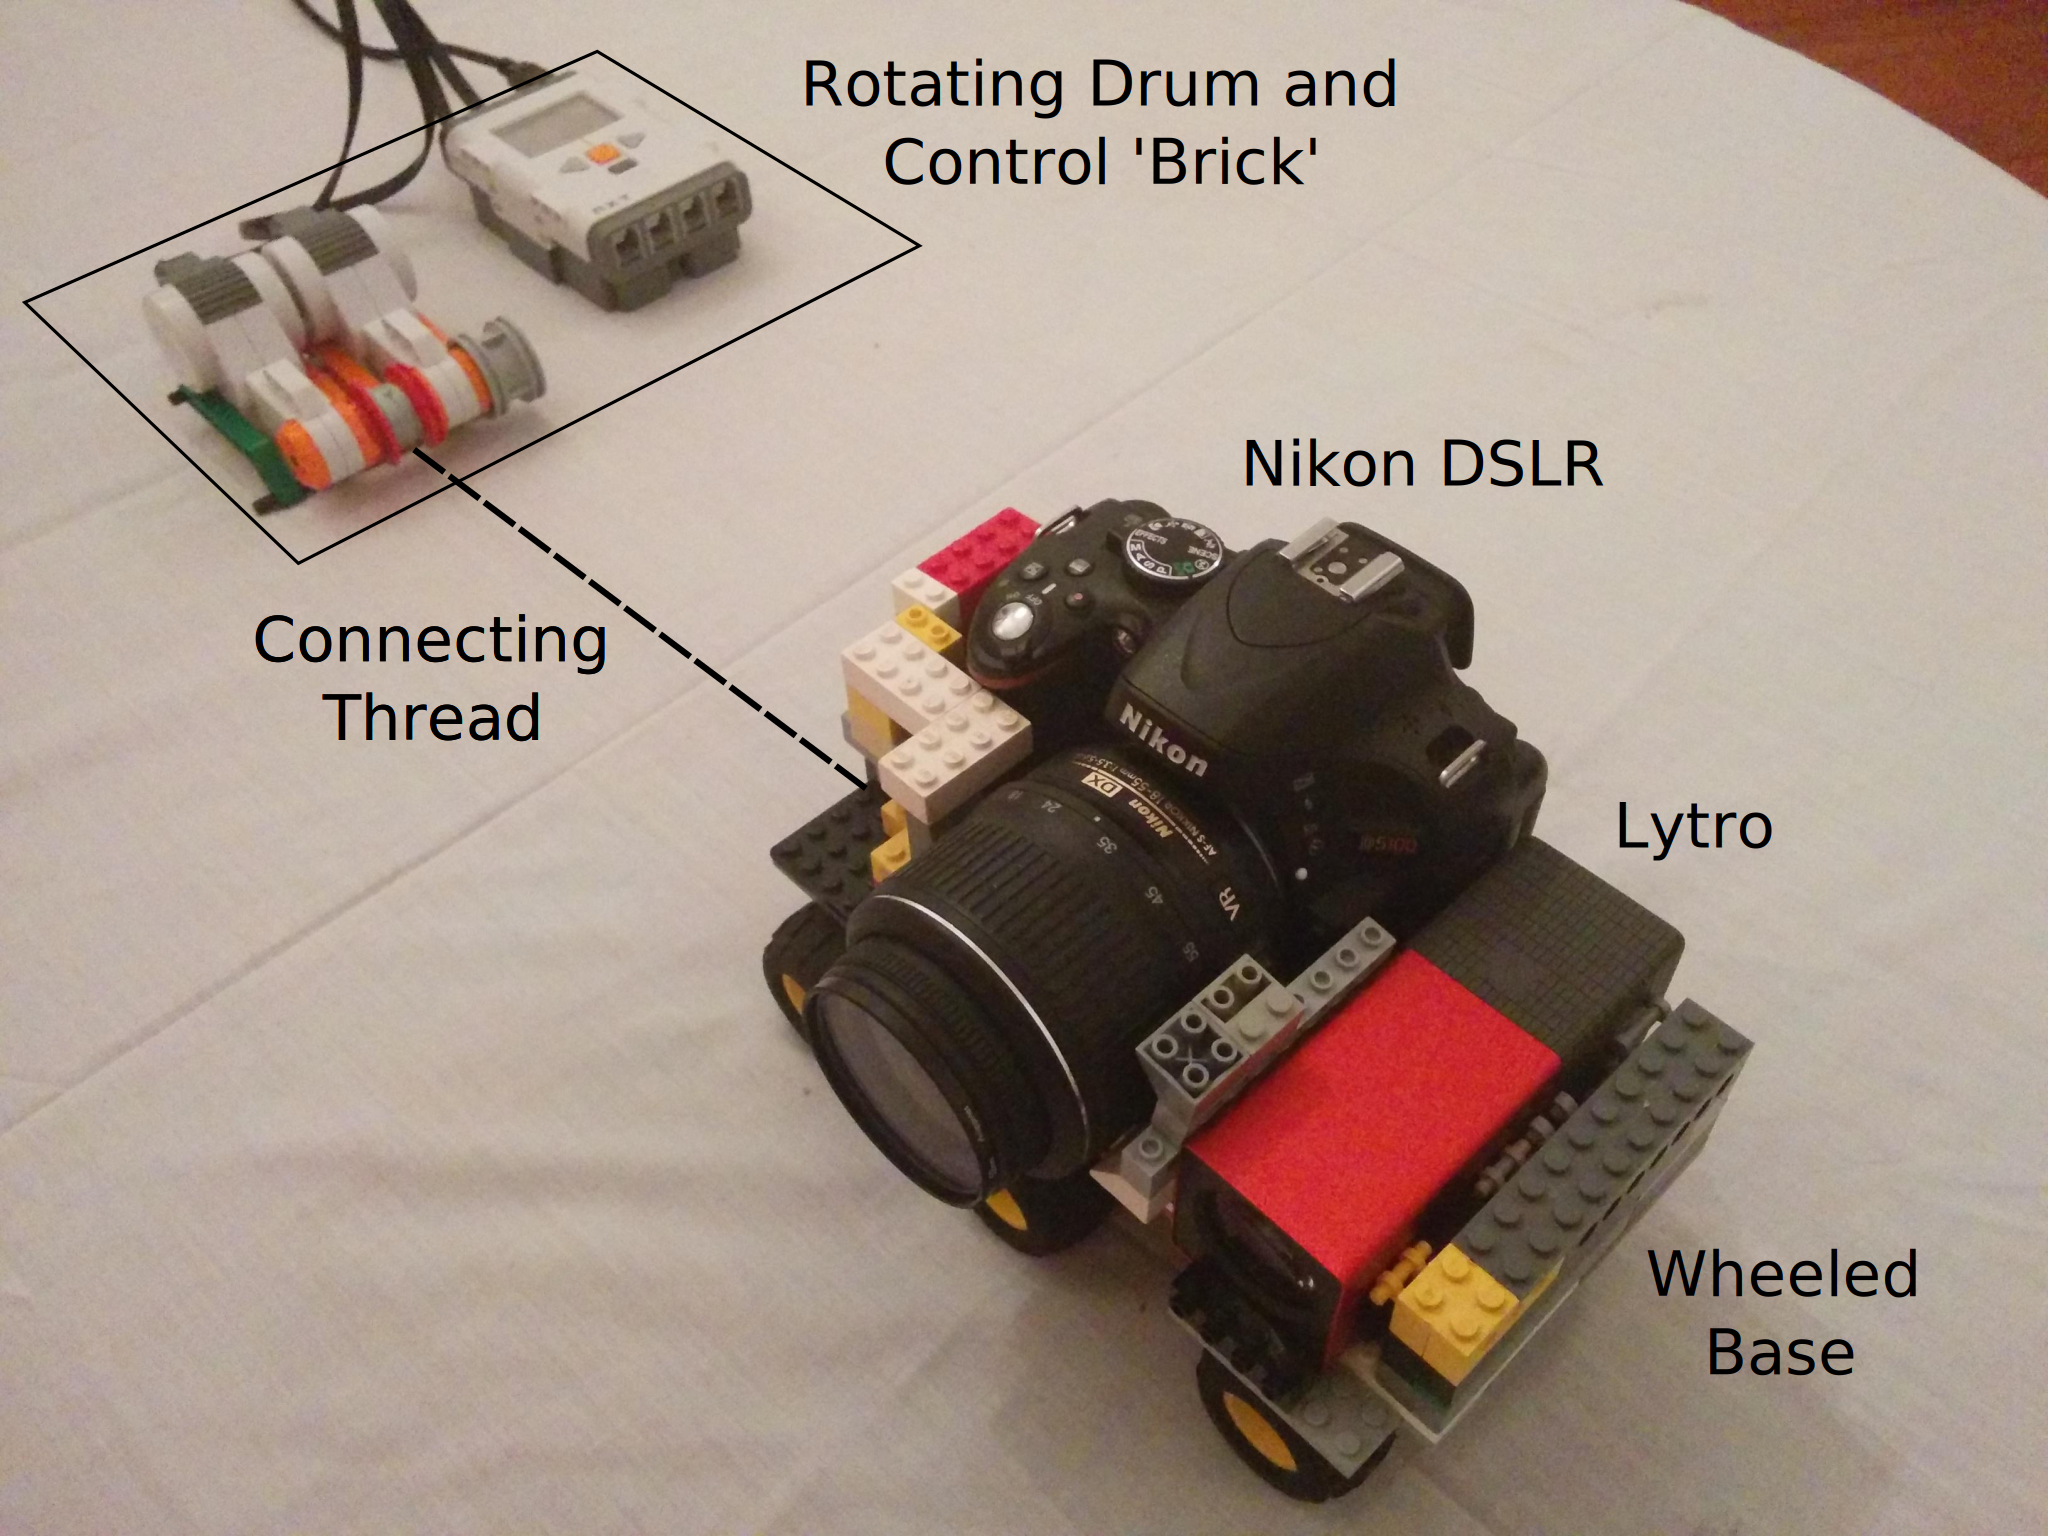
\includegraphics[width=\textwidth]{motion_platform}
\caption[Linear motion platform design]{Linear motion platform design}
\label{fig:motion_platform}
\end{figure}


\section{Scene Design}
\label{sec:scene_design}

Photographic scenes were set up in a room with no external facing windows to ensure the scene brightness could be controlled.
Three 60 watt incandescent static ceiling lights were used for ambient lighting in conjunction with a single 72 watt diffuse incandescent light source placed behind the linear motion platform carrying the cameras..
The 72 watt light source was placed facing front-on to the scene to reduce visible shadow size.
A plain white covering was placed on the working surface to reflect extra ambient light.

A large board was placed behind the scene to provide a constant background depth and scene elements were elevated using platforms where necessary.
The scenes used had a depth range (distance from the front of the Lytro camera to the background plane) of up to 50cm.
Figure \ref{fig:scene_description} shows the experimental scene configuration.

\begin{figure}[h]
\centering
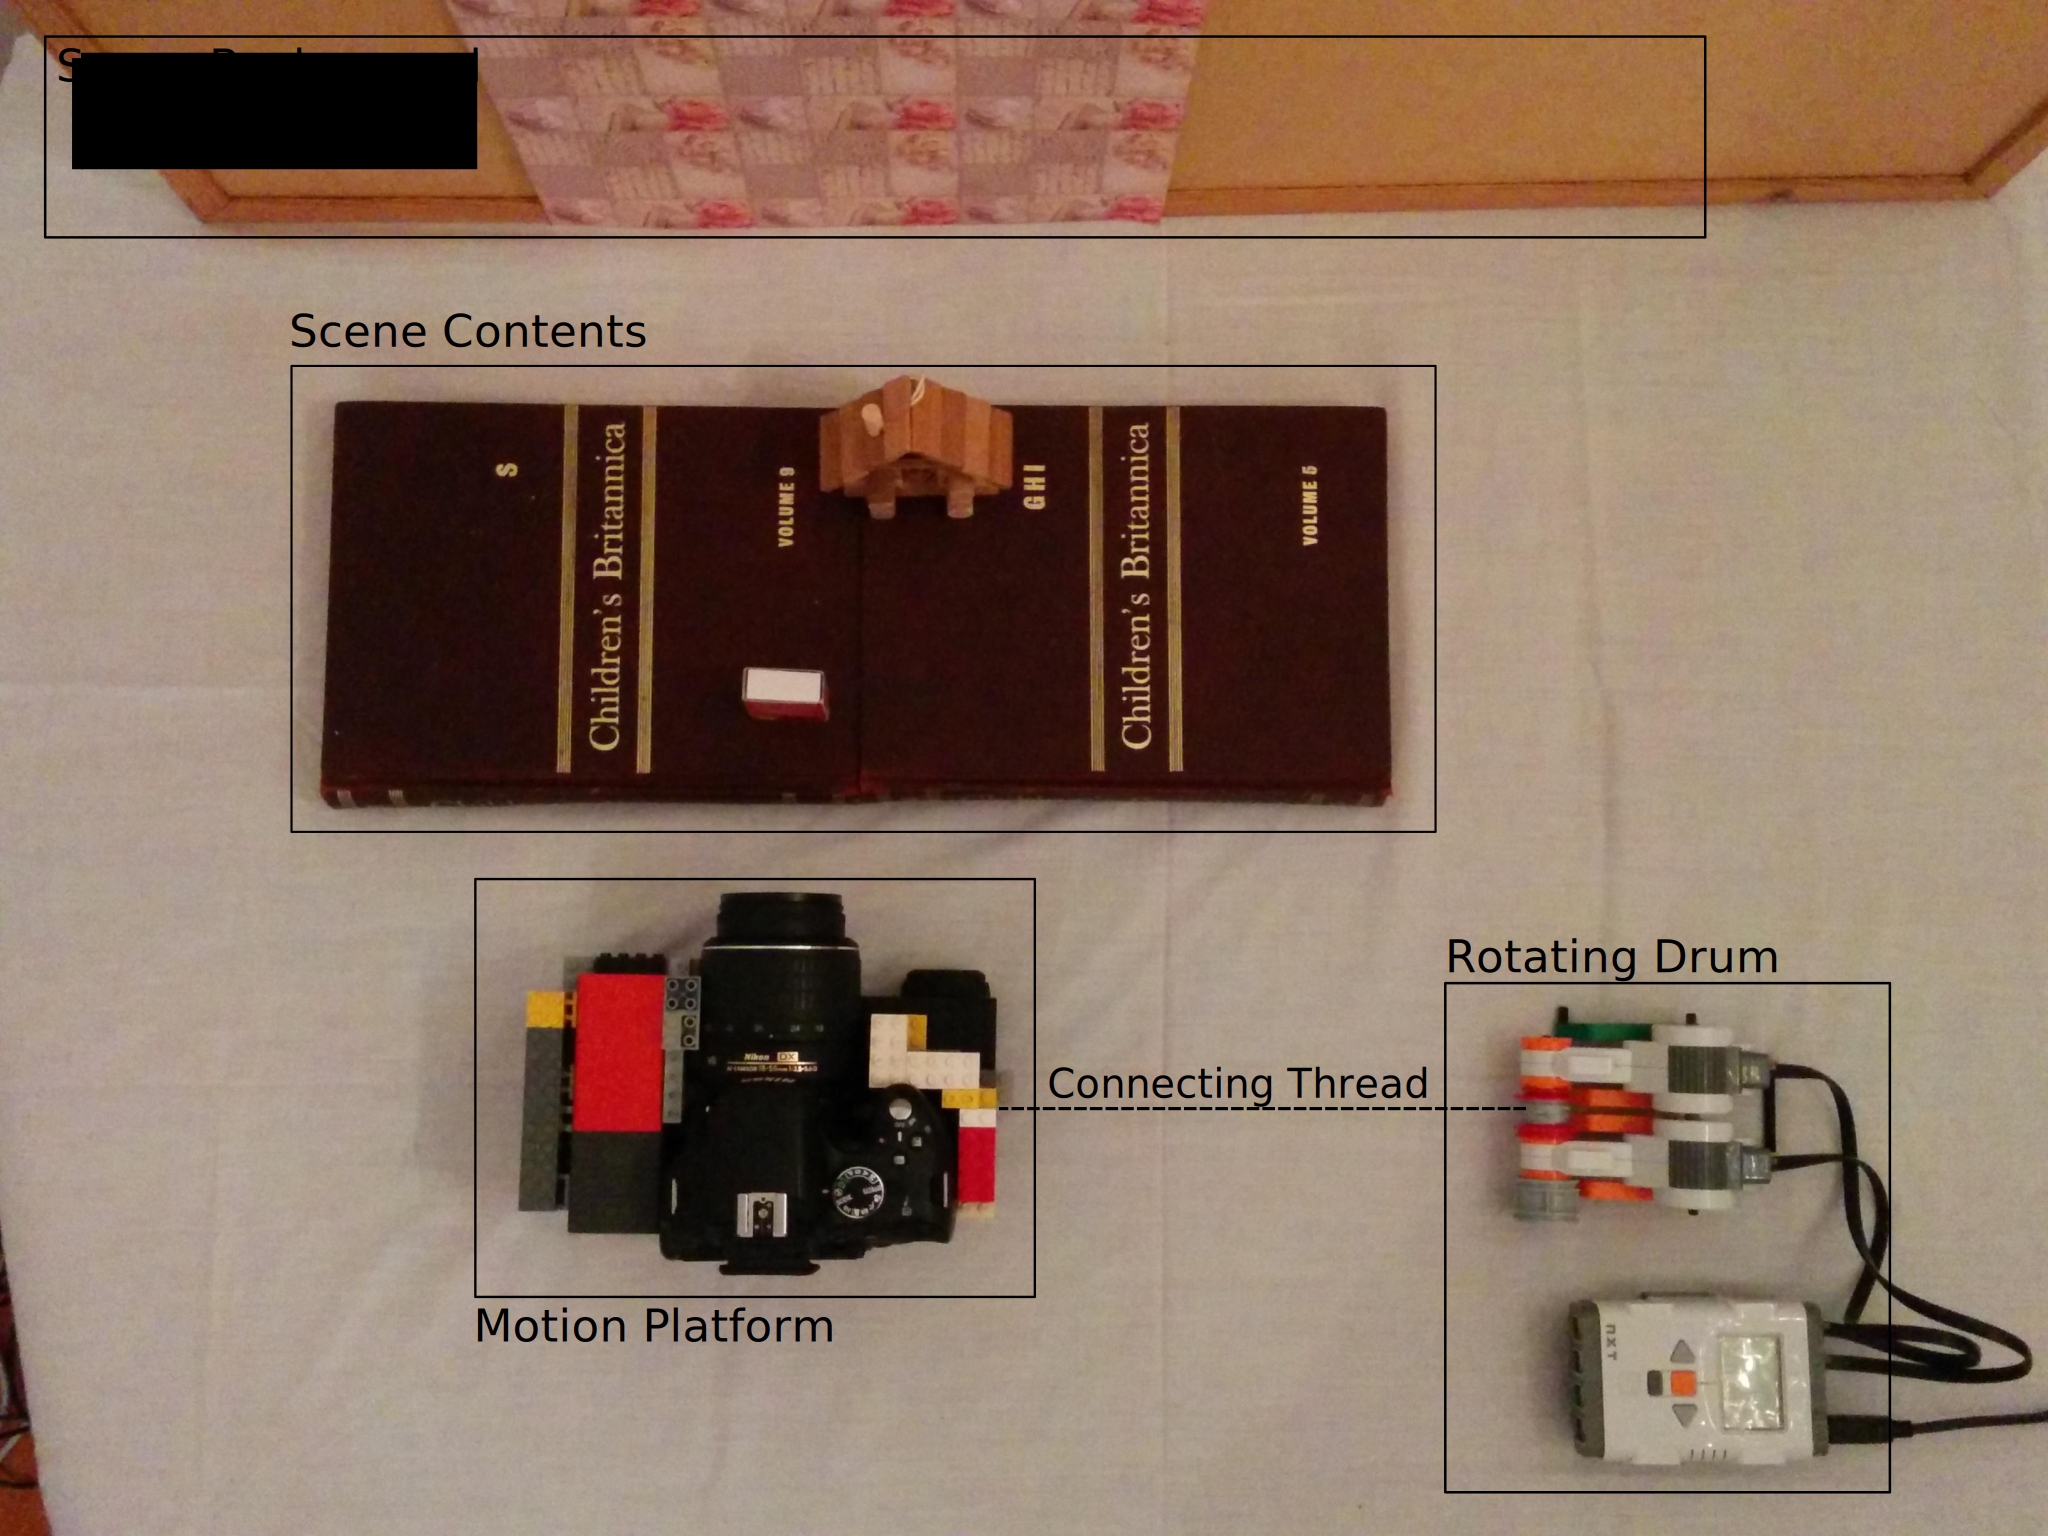
\includegraphics[width=\textwidth]{scene_contents}
\caption[Experimental scene layout]{Experimental scene layout, shown from above}
\label{fig:scene_description}
\end{figure}


\section{Image Capture}
\label{sec:image_capture}

A Lytro camera with firmware version 1.2.2 was used for the light field photography.
The Lytro camera was configured using the following settings.

\begin{table}[h]
\centering
\caption{Lytro Camera Settings}
\label{tab:lytro_settings}
\begin{tabular}{r | l}
Zoom & 1.0 \\
Creative Mode & Off \\
ND Filter & Off \\
ISO Sensitivity & Auto \\
Shutter Speed & As Required \\
Shutter Delay & 10s \\
\end{tabular}
\end{table}

The shutter delay was set to 10s to allow the motion platform to reach a stable velocity before the picture was taken.
Once the camera countdown was started, the motion platform was initiated from a Laptop running Matlab version R2009 and the RWHT Mindstorms Toolbox \cite{rwth2007toolbox}.

Images were transfered to an computer using the standard Lytro Desktop companion software (version 3.1.1 for OSX).
A 2011 model Apple Mac Book Air running OSX 10.9.3 was used for image processing.
Version 0.2 of the Light Field Toolbox \cite{dansereau2013toolbox} was used for light field manipulation and processing in Matlab.
The image decoding process used by the LF toolbox is described in \cite{dansereau2013decoding}.
Lytro \enquote*{.lfp} files were converted to raw image files and metadata files using the python-lfp-reader Python scripts (version 0.2) \cite{esfahbod2013python}, as per the Matlab LF Toolbox instructions \cite{dansereau2013toolbox}.

\section{Image Processing and Deconvolution}
\label{sec:image_processing_and_deconvolution}

The raw image files were read using the Matlab LF Toolbox, as described in \cite{dansereau2013toolbox}.
The Lytro depth maps were extracted from the Lytro desktop software image database using the python-lfp-reader Python scripts \cite{esfahbod2013python}.

Camera velocity was measured using the Lego Mindstorms motor encoders on the motion platform after initial calibration of the platform.

The exposure time and focal length were read from the Lytro image metadata, and a scaling factor for the Lytro focal length determined experimentally by comparing observed blur lengths with metric depths, using Equation \ref{eq:blur_width_simple}.

To de-blur the light field, all possible sup-aperture slices were taken and individually deconvoled once at every scene depth.
This was done using the Richardson-Lucy method due to it's comparatively short processing time and characteristically good performance.
The Matlab \enquote*{deconvlucy} command was used for the Richardson-Lucy de-blurring implementation.
The deconvoled sub-aperture images were then combined, using image masks computed for each depth map depth.
The deblurred sub-aperture images were combined such that the optimal PSF was used for each pixel within the final image.
This Matlab code for this process is fully described in Appendix XXXX.

[Figure or code listing XXXX here showing de-blurring process]

\section{Analysis}
\label{sec:analysis}

Two quantitative measures were used to compare de-blurred light fields.
A \enquote*{Q-Factor	} was computed to measure the increase in image sharpness and the Root-Mean-Square Error (RMSE) was estimated to measure the degree of noise amplification introduced by the deconvolution.

Without a ground truth image, a simple and well defined measure of \enquote*{image sharpness} is not easy to formulate, as evidenced by the complexity of image sharpness standards \cite{imatest2014sharpness}.
The original intention was to use the DSLR camera for capturing ground truth images, however due to the short depth range within the scene, the DSLR camera was unable to focus on all objects within the scene.
As such, a Q-factor had to be derived without access to a ground truth image.
The Q-factor definition used met this requirement and served to demonstrate the quantifiable recovery of high-frequency image content after de-blurring.

The Q-Factor used here was computed by summing absolute pixel intensities after applying a vertical Prewitt edge detection filter.
These sums were then normalised relative to the original blurred image Q-factor.
This had the effect of measuring the increase in the intensity of high-frequency components in the image.
Thus, the Q-factor we used was

\begin{equation}
Q = \frac{\sum_{x=1}^{W} \sum_{y=1}^{H} \left| (I \ast G)(x, y) \right|}
{Q_b}
\label{eq:q_factor}
\end{equation}

\noindent
where $Q_b$ is the Q-Factor for the original image (computed using the numerator of Equation \ref{eq:q_factor} only), $W$ and $H$ are the width and height of the image, $I$ is the de-blurred image, and $G$ is the Prewitt vertical edge detection kernel;

\begin{equation}
G = 
\begin{bmatrix}
1 & 0 & -1 \\
1 & 0 & -1 \\
1 & 0 & -1 \\
\end{bmatrix}
\label{eq:prewitt_filter}
\end{equation}

The vertical detection kernel was used due to the presence of horizontal motion blur in our images.
This Q-factor definition had the downside of also measuring noise content.
Thus, noisy images could potentially score higher than clean, sharp images.
To account for this, and provide a more balanced measure of de-blurring performance, the RMSE noise estimate was also used to compare de-blurred images.

The RMSE noise was estimated by converting the central sub-aperture image to grayscale, then manually cropping out a small (approximately 50x50 pixel) region known to be of constant color.
The RMSE was then computed using

\begin{equation}
R = \sqrt{ \sum_{x=1}^{W} \sum_{y=1}^{H} (I(x,y) - m)^2 }
\end{equation}

\noindent
where $W$ and $H$ are the width and height of the region respectively, $I$ is the region image and $m$ is the mean gray level within the region.
This metric gives an estimate of the additive noise content in the image prior to de-blurring, and an estimate of the noise (ringing and additive) in the image after de-blurring.



\chapter{Results and Discussion}
\label{chap:results_and_discussion}

\section{Experimental Results}
\label{sec:experimental_results}

Using the indoor motion platform described in Section \ref{sec:development_of_linear_motion_platform} and the experimental setup described in Section \ref{sec:scene_design}, images from three individual scenes with depths ranging up to \nicetilde0.4m were captured.
The motion platform velocity was controlled and was measured at $v_c = 0.021m/s$.
The Lytro exposure time was varied from 1/6.4s to 1/2s while the Lytro ISO setting was set to automatic to maintain scene brightness.

The Lytro depth maps were calibrated using the shallow depth range mapping described in Figure \ref{fig:depth_real_world_vs_lytro_response}.
The depth map data was then used to de-blur the light fields, using the technique described in Section \ref{sec:image_processing_and_deconvolution}.
For comparison, the light field images were also de-blurred using the Richardson-Lucy method, blind deconvolution and a simple regularized deconvolution implementation.
Each of the 2D deconvolution methods was applied in a simmilar manner to the depth-aware deconvolution, however a single PSF was used, computed at the median scene depth.

The computed Q-factors and estimated RMSE noise levels are shown in Tables \ref{tab:deblurred_light_field_q_factors} and \ref{tab:deblurred_light_field_rmse_estimates}.


\begin{table}[h]
\centering
\caption[De-blurred light field Q Factors]{
De-blurred light field Q Factors.
Increased high-frequency content is indicated by larger values (largest result in \textbf{bold}).
}
\label{tab:deblurred_light_field_q_factors}
\begin{tabular}[h]{r | c c c}
                & Milo          & House          & Bears         \\
\hline
Original        & 1.00          & 1.00           & 1.00          \\
Ours            & \textbf{2.26} & 1.56           & 1.68          \\
Blind           & 1.60          & 1.92           & 1.69          \\
Regularised     & 2.23          & \textbf{2.68}  & \textbf{2.53} \\
Richardson-Lucy & 1.62          & 1.93           & 1.69          \\
\end{tabular}
\end{table}


\begin{table}[h]
\centering
\caption[De-blurred light field RMSE Estimates]{
De-blurred light field RMSE Estimates.
Less image noise indicated by smaller values (smallest result in \textbf{bold}).
}
\label{tab:deblurred_light_field_rmse_estimates}
\begin{tabular}[h]{r | c c c}
                & Milo           & House         & Bears         \\
\hline
Original        & 3.96           & 2.72          & 3.18          \\
Ours            & \textbf{5.90}  & \textbf{3.94} & 4.15          \\
Blind           & 9.06           & 4.98          & \textbf{4.14} \\
Regularised     & 11.23          & 7.22          & 5.78          \\
Richardson-Lucy & 9.19           & 4.99          & 4.15          \\
\end{tabular}
\end{table}


Selected light field images of the three scenes are shown in Figures \ref{fig:results_milo_long_b} to \ref{fig:results_bears_short}, along with the respective depth maps, our results, and results from 2D deconvolution.


\begin{figure}[h]
\centering
\includegraphics[width=\textwidth]{results_milo_long_b.pdf}
\caption[De-blurring results - \enquote*{Milo} Scene]{
De-blurring results - \enquote*{Milo} Scene.
ISO Setting: 75, Exposure time: 1/2s.
a) Original blurred scene b) Lytro depth map c) Our de-blurred result, and results from 2D blind (d), regularised (e) and Richardson-Lucy (f) deconvolution.
Note that in (c) the text on the ground is sharp at all scene depths.
}
\label{fig:results_milo_long_b}
\end{figure}

\begin{figure}[h]
\centering
\includegraphics[width=\textwidth]{results_house_short.pdf}
\caption[De-blurring results - \enquote*{House} Scene]{
De-blurring results - \enquote*{House} Scene.
ISO Setting: 207, Exposure time: 1/6.4s.
a) Original blurred scene b) Lytro depth map c) Our de-blurred result, and results from 2D blind (d), regularised (e) and Richardson-Lucy (f) deconvolution.
Note the ringing in the background is more pronounced in (d)-(f) than in our de-blurred image (c).
}
\label{fig:results_house_short}
\end{figure}

\begin{figure}[h]
\centering
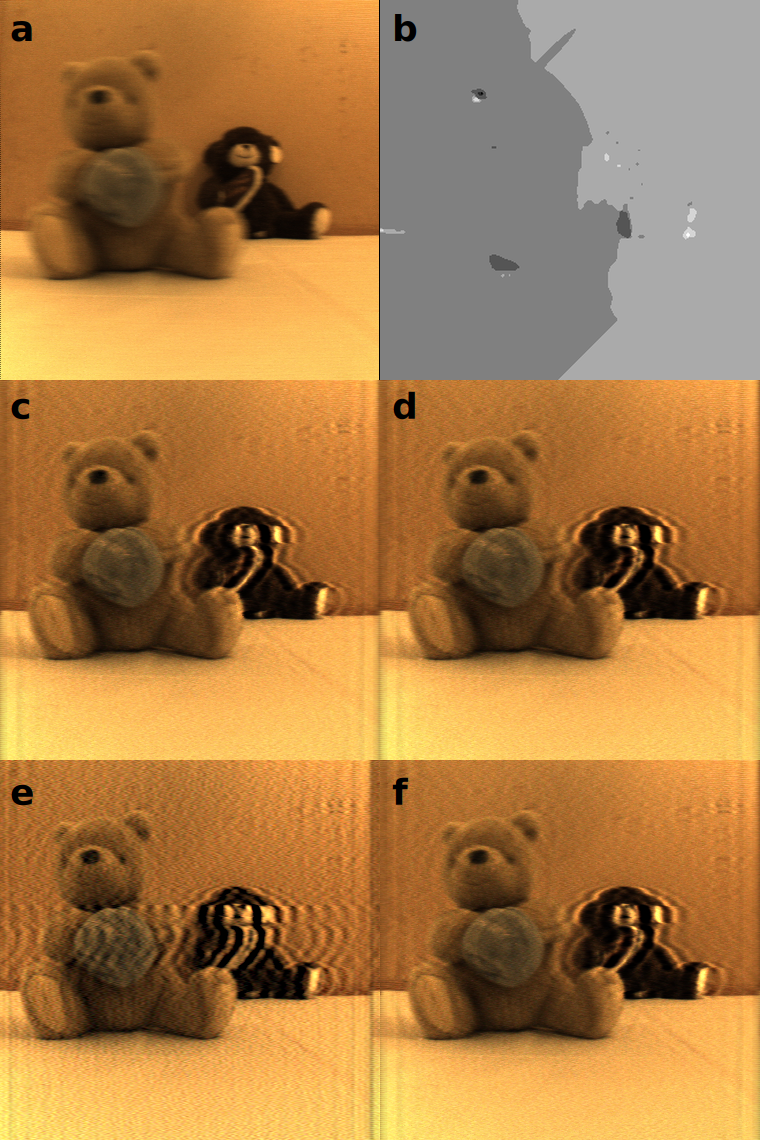
\includegraphics[width=\textwidth]{results_bears_short.pdf}
\caption[De-blurring results - \enquote*{Bears} Scene]{
De-blurring results - \enquote*{Bears} Scene.
ISO Setting: 113, Exposure time: 1/2s.
a) Original blurred scene b) Lytro depth map c) Our de-blurred result, and results from 2D blind (d), regularised (e) and Richardson-Lucy (f) deconvolution.
There is little difference between images (c) and (d-f) due to the lack of depth variation and the poor quality depth map.
}
\label{fig:results_bears_short}
\end{figure}



\section{Discussion}
\label{sec:discussion}

Table \ref{tab:deblurred_light_field_q_factors} shows that the Q factor increased for each test scene using our de-blurring method.
Additionally, the Q-factors from the 2D deconvolution methods increased for each scene.
This indicated that after de-blurring, the light field images contained a greater proportion of high-frequency content in the horizontal direction.
This can be seen visually in the de-blurred light field images.
Note that, as stated in section \ref{sec:analysis}, the Q-factor does not discriminate between high-frequency content due to a lack of motion smear and high-frequency content due to false ringing edges created by noise amplification.
This is highlighted for example in Figure \ref{fig:results_milo_long_b}e, where a Q-factor of 2.23 was observed, yet the image is completely corrupted by ringing artifacts, instead of being a sharp image of the ground truth scene.

For this reason the RMSE noise estimate was used as a second quantitative metric.
The RMSE noise figures in Table \ref{tab:deblurred_light_field_rmse_estimates} indicate that our de-blurring method raised the RMSE noise less than the 2D deconvolution methods for the \enquote*{Milo} and \enquote*{House} scenes, and raised the RMSE noise level by a comparable amount for the \enquote*{Bears} scene.
The RMSE values for the regularised de-blurring method are larger than those for all other methods, reflecting the more visible presence of ringing in Figures \ref{fig:results_milo_long_b}e, \ref{fig:results_house_short}e and \ref{fig:results_bears_short}e.
Our de-blurring method's RMSE noise performance in the \enquote*{Bears} scene was comparable to that of the 2D deconvolution methods due to the lack of significant depth difference in the scene, and the low quality depth map present for that scene.
The poor quality depth map was in this case caused by a lack of scene structure in all parts of the scene.
As stated in section \ref{sec:experimental_results}, the 2D deconvolution methods used a single PSF computed from Equation \ref{eq:blur_width_simple} using the median scene depth.
Thus, for the \enquote*{Bears} scene, the PSF used for the 2D deconvolution methods was similar in width to the PSFs used by our method, the result being that our method showed only slightly better or equal performance when compared with 2D deconvolution methods.

Figure \ref{fig:results_milo_long_b} most clearly shows the benefit of our method over 2D deconvolution methods; for example the text on the ground is de-blurred continuously though all scene depths, a feat which is impossible for 2D deconvolution methods to do.

In Figure \ref{fig:results_house_short} the benefit of our method is less pronounced, however ringing in the background of the scene is more pronounced in the 2D deconvolution cases.
This reflects the fact that a single PSF was used to de-blur a scene with varying degrees of motion blur.
In this case, the PSF used was sub-optimal for the degree of motion blur present in the background, and thus introduced excess ringing.

Figure \ref{fig:results_bears_short} again shows little difference between our method and the 2D deconvolution methods.
In this case, as explained above, this is due to the presence of only two major depth planes in the scene and the poor quality depth map.
Looking closely at the background bear's face reveals sharper features in our result than in the other cases.

Finally, note that the original purpose of the DSLR camera was to capture ground-truth sharp images for comparison with the light field images.
This would have allowed more accurate RMSE and Q-factor metrics to be computed.
Unfortunately due to the shallow depth range used in the experiment the DSLR was unable to bring all objects within the scene into focus.
For this reason, the DSLR images were not used in the final comparisons.
The DSLR was left in-place for all images to ensure the motion platform velocity calculations were correct, however the actual DSLR images were not used at all.

\section{Implications}
\label{sec:implications}

By analysing the projective geometry camera equation (Equation \ref{eq:camera_projection}), we have shown that metric depth measurements can be combined with knowledge of a camera trajectory and camera intrinsics to compute 3D point-spread functions.
This was verified experimentally, as shown in Figure \ref{fig:blur_vs_depth}.
We suggest that a 3D PSF is better than a 2D PSF as it allows for depth-aware deconvolution.
This type of deconvolution allows an optimal PSF to be used for all parts of an image, reducing ringing artifacts and increasing the quality of the de-blurred image.
For a practical demonstration of depth-aware deconvolution, we investigated the possibility of de-blurring light field images from a commercial Lytro camera.

Our initial experimental work suggested that Lytro depth maps are consistent for light field images with similar overall depth range.
This implies that if a rough estimate of the scene depth can be made, Lytro depth maps can be calibrated using a piecewise linear mapping.
We suggest that user-supplied scene information (e.g. from the \enquote*{scene} setting on a commercial camera), a cheap depth sensor such as an IR or ultrasound based focal-range sensor or \emph{a-priori} knowledge of a robotic operating environment can be used to this end.

The experimental results of our de-blurring tests show that linearly motion-blurred light field images from a Lytro camera can be de-blurred at all scene depths.
In order to do this, a rough estimate of the scene depth range is needed to calibrate the Lytro depth data, and the camera velocity, exposure time and focal length need to be known.
This technique however is not limited to Lytro images.
Our depth-aware deconvolution method could also be applied to images from any RGBD sensor that can provide calibrated depth maps, e.g. the Microsoft Kinect sensor. 
Using the Lytro camera is beneficial in this regard as de-blurred light field data can be obtained, opening more possibilities for computational photography.

Future practical applications of depth aware deconvolution include improving consumer satisfaction with hand-held light field and RGBD camera devices by de-blurring camera shake.
This will be more widely applicable in the near future, given that consumer smartphones are beginning to be equipped with depth-sensing capabilities \cite{google2014lensblur, google2014tango}.

Depth-aware deconvolution also has potential benefits for forensic and photo-restoration applications, even where depth information is not readily available.
For example the specification of a depth map could potentially be performed through interactive user input with one or more images \cite{sinha2008interactive}.
By exploiting user supplied \emph{a-priori} information about the content of a photo in this way, it may be possible to perform depth-aware deconvolution even on photos where a depth map is not available. 

Finally, we anticipate that depth-aware deconvolution will have benefits in robotic navigation and computer vision applications.
Robotic systems have many attributes that make them suitable for depth-aware deconvolution; often camera intrinsics are known, and the exposure time of images can be obtained, camera trajectory will likely be known thanks to motion encoders or other robotic sensors, and increasingly, more robotic systems are incorporating highly capable depth sensors.
Light field sensors such as the Lytro have the potential to be powerful tools for robotic systems, and by demonstrating the ability to de-blur a light field image, it is hoped that the performance of robotic light field computer vision systems can be improved, e.g. in low-light operating environments where motion blur is more likely.


\section{Limitations and Future Work}
\label{sec:limitations_and_future_work}

The work presented here has several limitations relating to the experimental method, the volume of data used and the types of light field images tested.

Our de-blurring method was demonstrated with linear motion blur only.
Equation \ref{eq:camera_projection} can equally be applied to compute a 3D PSF for optical-axis rotational camera motion, or even generalized camera trajectories.
Future work could explore if these PSFs can be used in the same way for de-blurring.

In the experiments performed the camera velocity used to compute the PSF was supplied \emph{a-priori}.
In a robotic system this information could potentially come from encoders, an inertial measurement unit or other velocity sensors.
Alternately, future work could explore the possibility of using blind deconvolution methods to simultaneously recover the camera velocity \emph{and} high-frequency image details.

The images used for in these experiments were all captured in a controlled environment.
Real-world implementations of this de-blurring method would need to be tested for robustness against lighting and other scene variations.

Light field pixel confidence maps are available in the Light Field Toolbox.
The Lytro desktop software also supplies depth confidence maps along with the depth data.
Neither of these sources of information were utilised in the experiments performed here.
Future work could look at integrating this data into the de-blurring process.
This could be used as a means for suppressing noisy regions of the light field, or regions where there is little confidence in the light field depth map.

Although many light field images were analysed while developing the depth-aware deconvolution method, only three scenes were used for the final analysis.
Future work could look at confirming the results found in this experiment by collecting more data.
More tests should also be performed at other scene depth ranges beyond 40cm.

The Lytro camera was the only light field camera used in this experiment.
The Lytro generates a light field with a specific dimensionality; for example Lytro light field images have a much larger spatial resolution than angular.
Future work could explore the use of other light field cameras.
More generally, light fields with other shapes (e.g. more angular resolution) could be tested with the depth aware deconvolution method.

Currently, technological limitations dictate that light field de-blurring is an \enquote*{off-line} process.
The Lytro desktop companion software must be used to download light field images before they can be processed, preventing any real-time robotic use of Lytro cameras.
Future work could look into reverse-engineering the Lytro camera USB or Wifi download protocols.
This would potentially allow Lytro cameras to be integrated into real-time mobile robotic systems.

Additionally, the de-blurring implementation shown here is computationally intensive.
To implement depth-aware deconvolution in a real world system (robotic or otherwise) the de-blurring process would need to be optimised using standard computer science methods.
The possibility of using GPU-based parallel processing methods could also be explored in future research.

For simplicity these experiments focused only on global motion blur caused by camera motion.
Future work could look into individual object blur, and applications for selectively de-blurring isolated objects in a scene.

As shown in section \ref{sec:light_field_depth_estimation}, the presence of motion blur reduces the quality of the light field depth estimation.
These depth maps are critical for depth-aware deconvolution, and are also a major benefit of using light fields generally.
Several possibilities for future work exit regarding the light field depth maps.
Techniques for more robust, blur-invariant light field depth estimation are needed.
Alternately, the method presented here has the potential to be adapted to an iterative form,
An initial de-blurring pass could allows a better depth estimation, followed by another de-blurring pass etc.

Finally, insufficient data was collected to fully quantify the Lytro depth map response function.
Further research with ground truth depth data is needed to better understand the limitations and behavior of the Lytro depth maps, particularly in uncontrolled real-world scenes.



\chapter{Conclusion}
\label{chap:conclusion}

\begin{itemize}
\item Mini version of aims and discussion
\item The contributions of this thesis are...
\end{itemize}

The aim of this experimental work was to investigate means for de-blurring light field images, with robotic applications of these images in mind.
In Section \ref{sec:light_field_theory} we covered the relevant background regarding the development of the Plenoptic theory and practical light field cameras.
The formation of motion blur in a camera was discussed in Section \ref{sec:motion_blur_formation}, and Equation \ref{eq:blur_width_simple} derived that gives the degree of linear motion blur present for a point source a given distance from a translating camera.
This equation was verified experimentally using the central sub-aperture slice from a Lytro light field image, indicating that depth-aware deconvolution should be possible given calibrated depth data, and knowledge of the camera intrinsics and motion.
A review of deconvolution de-blurring methods was given in Section \ref{sec:image_deblurring}, and a means for applying deconvolution to a light field image proposed.
Finally, Section \ref{sec:light_field_depth_estimation} described the extraction and limitations of depth map data from a light field, and outlined a means for calibrating Lytro camera depth maps.

An experiment was designed to test the depth-aware deconvolution method, and the experimental method was described in Chapter \ref{chap:experimental_method}.
This included the design of a controlled scene and linear motion platform, image capture and processing, and the formulation of quantitative de-blurring quality metrics.

The experimental results were discussed in chapter \ref{chap:results_and_discussion}.
The quantitative metrics indicated that depth aware deconvolution results in a greater recovery of high-frequency content in an image, and that the ringing noise introduced was less than traditional 2D deconvolution methods.
The benefit of depth aware deconvolution was most pronounced for scenes where an accurate depth map could be recovered.
Lack of scene structure and lack of significant depth variation in the scene were highlighted as two causes for degraded depth map performance, and subsequently degraded de-blurring performance.

The depth-aware deconvolution method will likely have applications in improving user satisfaction with light field and RGBD camera performance in the future.
Furthermore, it was suggested that in some cases interactive user input may be used to improve de-blurring performance on images even when a depth map was not originally present.
Finally, it is expected that depth aware deconvolution will have benefits for robotic navigation and computer vision applications going forward.

Several areas for future research were outlined, including extending the experimental proof to arbitrary camera trajectories, testing the results in a non-controlled environment, integrating the available light field confidence data in the method, collecting more data to verify the results and finding means for more accurate depth recovery from the light field.


\bibliographystyle{unsrt}
\bibliography{bibliography/thesis_bibliography}

\end{document}